%        File: test.tex
%     Created: Thu Jul 29 09:00 PM 2021 E
% Last Change: Thu Jul 29 09:00 PM 2021 E
%

\documentclass[border=2pt]{standalone}
\usepackage{pgfplots}
\usetikzlibrary{calc}
\usepackage{amsmath}

\begin{document}
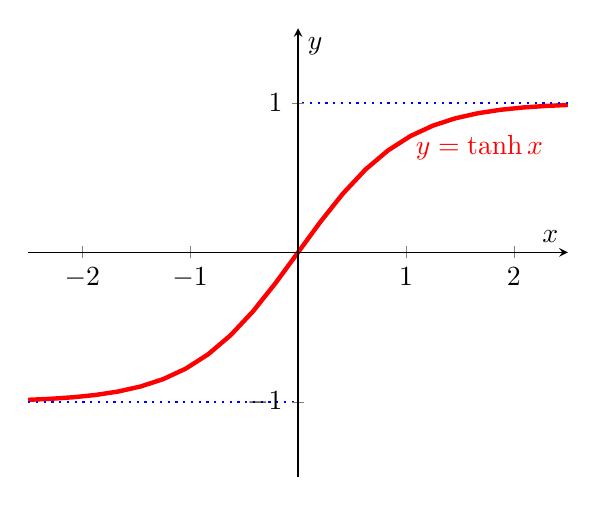
\begin{tikzpicture}
\begin{axis}[
    xmin=-2.5, xmax=2.5,
    ymin=-1.5, ymax=1.5,
    axis lines=center,
    axis on top=true,
    domain=-2.5:2.5,
    ylabel=$y$,
    xlabel=$x$,
    ]

    \addplot [mark=none,draw=red,ultra thick] {tanh(\x)};
    \node [right, red] at (axis cs: 1,0.7) {$y = \tanh x$};
    
    %% Add the asymptotes
    \draw [blue, dotted, thick] (axis cs:-2.5,-1)-- (axis cs:0,-1);
    \draw [blue, dotted, thick] (axis cs:+2.5,+1)-- (axis cs:0,+1);
\end{axis}
\end{tikzpicture}
\end{document}
\end{document}


